\documentclass{muthesis2017}
\setcounter{secnumdepth}{4} % make subsubsection have numberings
\usepackage{graphicx}
\usepackage{latexsym}
\usepackage{amsmath}
\usepackage{amsthm}
\usepackage{url}
\usepackage{textcomp}

\usepackage{caption,setspace}
\captionsetup{font={stretch=1.5}} % make the table,figure captions also have 1.5 linespacing

\usepackage[flushleft]{threeparttable}
%\usepackage{notoccite}
\graphicspath{ {../figures/} } % path to figures; you can put multiple of them. Just put them in separate brackets
\newcommand\mathplus{+}

\makeatletter
\renewcommand{\@dotsep}{10000} % set distance between dots to make it disappear in the table of contents
\setlength{\@fptop}{0pt}
\setlength{\@fpbot}{0pt plus 1fil}
\makeatother

% title of thesis -- nouns and stressed words should begin
\title{Thesis title}

\author{Firstname Lastname}


\candidate{Angkana Huang} % your name (without title)

\candidatetitle{Miss.\ } % Mr.\ Miss.\ or Ms.\ 

\degree{MSc} % default is MSc

\subject{Computer Science} % subject area of your thesis 

%\submissionyear{} % default is current year -- but maybe you will
                  % want to print it out again next year

%\isbn{974-04-xxxx-x} % remember to replace the x's when you know the number

% information for page i (advisors)

% NOTE: to avoid hyphenation in names on the abstract page, try
% putting the name which is hyphenated inside \mbox{ }
\majoradvisor{Apirak Hoonlor} % name of supervisor (without title)
% default title is Lect.\
\majoradvisortitle{Lect. } % Dr.~ or Asst.~Prof.~ or Assoc.~Prof.~ or Prof.~  
\majoradvisorletters{Ph.D.} % Ph.D. or Dr.rer.nat.
\majoradvisorsubject{Computer Science} % subject in which advisor obtained last degree

\coadvisor{Peter Haddawy} % name of co-advisor
\coadvisortitle{Prof. } % title of co-advisor
\coadvisorletters{Ph.D.} % Ph.D. or Dr.rer.nat.
%\coadvisorstatus{Major advisor} % default is co-advisor but you might want
				% to classify him/her as a joint major advisor
\coadvisorsubject{Computer Science} % subject in which co-advisor obtained last degree

\coadvisorII{Damon W. Ellison} % in case you have two co-advisors
\coadvisorIItitle{MAJ }
\coadvisorIIletters{Ph.D.}
\coadvisorIIsubject{Molecular Microbiology and Microbial Pathogenesis}

%\coadvisorIII{} % in case you have three co-advisors
%\coadvisorIIItitle{}
%\coadvisorIIIletters{}
%\coadvisorIIsubject{}

\programchair{Asst. Prof. Boonsit Yimwadsana} % chair of your degree program
\programchairqual{Ph.D. (Electrical Engineering)} % qualifications of program chair
\faculty{Information and Communication Technology}
%\facultyI{Information and Communication} % Faculty name is not too long
%\facultyII{Technology} % Faculty name is too long to fit in one line

% default graduate studies dean is Prof.~M.R.~Jisnuson Svasti, Ph.D.
\graduatestudiesdean{Prof. Patcharee Lertrit,\\M.D., Ph.D. (Biochemistry)}
%\GSDqual{Ph.D.} % this is no longer used
%\GSDstatus{Acting} % in case the dean is away and you need to put
		   % `Acting Dean' on the form 

% information for page ii (exam committee)

\submissiondate{January 5, 2017} % date of submission

\chair{Asst. Prof. Thanawin Rakthanmanon}
\chairqual{Ph.D. (Computer Science)} % qualifications of chair
%\memberI{Lect. Sudsanguan Ngamsuriyaroj} % use this if the major advisor is not present at the exam
%\memberIqual{Ph.D.} % qualifications of 1st member
%\memberIqual{Ph.D. (Computer Science and Engineering)} % qualifications of 1st member
%\memberII{Assoc. Prof. Damras Wongsawang} % use this if the co-advisor is not present at the exam
%\memberIIqual{Ph.D.} % qualifications of 2nd member
%\memberIIqual{Ph.D. (Information Engineering)} % qualifications of 2nd member
\memberIII{MAJ Damon W. Ellison} % 3rd member
%\memberIIIqual{Ph.D.} % qualifications of 3rd member
\memberIIIqual{Ph.D. (Molecular Microbiology and Microbial Pathogenesis)} % qualifications of 3rd member
%\memberIV{} % 4th member
%\memberIVqual{} % qualifications of 4th member

\facultydean{Assoc. Prof. Jarernsri L. Mitrpanont}    % default is Prof.~Prasert Sobhon
\FDqual{Ph.D. (Computer Science)}         % default is Ph.D.
%\FDstatus{Acting} % in case the dean is away and you need to put
		   % `Acting Dean' on the form 

% information for page iv (ABSTRACT)

\candidatenumber{ 5837702 ITCS/M}
%\major{} % major of thesis (not necessary if the same as subject)
\keywords{RECOMMENDATION SYSTEM / INFORMATION RETRIEVAL /} % 1st line of keywords
\keywordsII{BIOINFORMATICS} % 2nd line of keywords
%\keywordsIII{ /  / } % 3rd line of keywords

% information for page v (THAI ABSTRACT)

\thaisubject{วิทยาการคอมพิวเตอร์} % thai name of degree subject
\thaititle{การแนะนำเครื่องมือทางชีวสารสนเทศโดยอิงหลักฐานทางการใช้งาน} % title of thesis in thai
\thaicandidate{นางสาวอังคณา หวัง} % your name in thai
\thaimajoradvisor{อาจารย์อภิรักษ์ หุ่นหล่อ} % Thai name of advisor (if they are Thai)
%\thaicoadvisor{} % Thai name of co-advisor (if they are Thai)
% you might need to put the individual (first and last) names
% inside \mbox{} to stop them being split by the word-breaking routine

%\thaicoadvisorII{} % Thai name of 2nd co-advisor (if they are Thai)

% information for Biography

\dateofbirth{15 June 1986} % your date of birth
\placeofbirth{Bangkok, Thailand} % province and country of birth
\firstdegreeinstitution{Chulalongkorn University} % where you did your first degree
\firstdegreeyears{2004--2008} % years for 1st degree
\firstdegree{Bachelor of Industrial Design} % default is Bachelor of Science
\firstdegreemajor{Ceramics} % first degree major
%\longfirstdegree % necessary if you want the subject on the next line
%\preinstitution{Asian Institute of Technology, 1993--1994} % details of place you went before present degree if
		  % it wasn't your 1st degree
%\preinstitutionLnII{Master of Engineering (Computer Science)} % 2nd line of details
%\preinstitutionII{} % details of 2nd place you went before present degree
%\preinstitutionIILnII{} % 2nd line of details
\years{2015--2016} % years taken to do your present degree
\postinstitution{Mahidol University} % details of place where you continued your study for your
		   % present degree
%\postinstitutionLnII{} % second line of details
%\scholarship{} % details of 1st scholarship
%\scholarshipLnII{} % 2nd line of details (if necessary)
%\scholarshipLnIII{} % 3rd line of details (if necessary)
%\scholarshipII{} % 2nd scholarship
%\scholarshipIILnII{}
%\scholarshipIILnIII{}
%\scholarshipIII{}  % 3rd scholarship
%\scholarshipIIILnII{}
%\scholarshipIIILnIII{}
%\scholarshipIV{}  % 4th scholarship
%\scholarshipIVLnII{}
%\scholarshipIVLnIII{}
\position{Data Analyst} % present position
\workplace{Department of Virology, USAMD-AFRIMS} % location 
\workplaceLnII{315/6 Rajvithi Road, Bangkok, Thailand} % second line of location
%\homeaddress{} % your home address if you do not have a position
%\homeaddressLnII{}
%\homeaddressLnIII{}
\email{AngkanaH@afrims.org} % the email address at which you can be contacted after you have left


         

\begin{document}

\maketitle

\linespacing{1.5}
\acknowledgements{You acknowledgement goes here.}

\abstract{%
\linespacing{1.2} % change the linespacing to fit the abstract in the allotted space
Your abstract goes here.} % point to english abstract.tex
% \thaiabstract{ภาษาไทย} % the Thai abstract doesn't work. Have to manually do it in Word. But leave this here so that the page number runs correctly.

\tableofcontents
\listoftables
\listoffigures

% your thesis goes here!
\chapter{Introduction} \label{chap:intro}

\section{A tribute to the former contributors}
The class styles used here were altered from Ekasit Kijsipongse's version in 2009 \cite{EkasitMuThesis}.
His work was based on the former work of Michael A. Allen in 2006 \cite{allenMuThesis}.
The changes made were based on the actual issues encountered at the format check in Salaya during February 2017.
This work here, including all of the just mentioned, are NOT the official templates from Mahidol University. Indeed, if there was one, we wouldn't have to do this in the first place.


\section{How to use the LaTeX template} \label{sec:use}
It will be best appreciated if you fork the repository and submit a pull request when you made improvements to it.
Hopefully some day, the future graduate students of Mahidol will be able to focus totally on the research rather than the formatting. As we all know, \textit{format check is not fun} and many times, time and resource consuming.


\subsection{Folder for source TEX files} \label{use:source}
I personally find the temporary files created during the PDF rendering process messy. Therefore, I keep my source files in a separate directory and run a script which copies them into the \textbf{mess} directory each time the PDF is being rendered as detailed in Section \ref{use:render}.

\subsection{Folder for figures} \label{use:fig}
The \textbf{figures} directory is placed in the core directory (Figure \ref{fig:screenshot}).

\begin{figure}[!htpb]
    \centering
    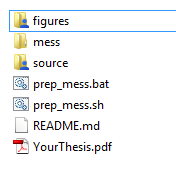
\includegraphics[width=.4\textwidth,keepaspectratio]{dirshot} % it understands PNG so the extension is omitted
    \caption{A screenshot of the core directory \cite{hatioMuThesis}} % if you took the image from somewhere, cite it
    \label{fig:screenshot}
\end{figure}


\subsection{Rendering the PDF} \label{use:render}
The rendering process is simple. Run the \textit{prep\_mess.bat} is you are running Windows, or run the \textit{prep\_mess.sh} if you are on Mac or Linux. The code starts with copying all the source files to the \textbf{mess} directory, do the first render to position all the components, do the second render to give the numberings to everything (e.g. the figure number, the table number, the reference number), and the last render to put the numbers into the refering places. After all, the \textit{main.pdf} is generated in the directory and moved to the core directory (its parent directory) changing it into the predefined name (\textit{YourThesis.pdf} is the default).



\section{Lessons learnt from the past}
\vspace{4.7ex}
\subsection{Subsections right after section}
Generally, the spacing between the text and the sections/subsections works fine.
However, for writing styles where the section is immediately followed by the subsection, the format requires that the section MUST be followed by one empty line before anything follows, including the subsection.
To do that a vertical space is manually addeded here (note the \textit{vspace}).


\subsection{Numbered and non-numbered lists}
Typically, LaTeX users would use \textit{enumerate} to make number lists. However, the Mahidol format checker insists that we have the indents as if each item in the list was a paragraph. The same applies for non-numbered lists. So I ended up manually doing them as below. If someone cool forked this and can fix the class file (.cls) such that we can do it the LaTeX way again, that would be awesome.

Example of numbered list:

1. First item: you won't notice what's the difference between this and enumerate unless you have a long, long text per item. Then, it will become evident.

2. Second item

3. Third item


Example of non-numbered list:

-- Item: The situation is the same for these bullet points. The moment you exceed one line per bullet, you will see why we need to do it this way.

-- Item: I know it looks highly awkward but this is what they want. And if you do not follow, you will end up not graduating, you know?

-- Item

-- Item

\newpage % manually put the following to a new page
\subsection{Subsubsections, equations, tables and figures}
The things binded together in this subsection will look awkward to you.
It is purposefully done this this way to demonstrate the points made in them. So please bear with it.

\subsubsection{Subsubsection}
\hspace{2cm}Text in the subsubsection has to be 4cm from the left margin (so manually added 2 more cm here).

\subsubsection{Equations}
\hspace{2cm}Placing the where clause outside the equation tag (treating as regular paragraph text) is alright.

\begin{equation} \label{eq}
P_{f,1}^{m,n} = C(F_{m,n}^f) / C(L_{m,n})
\end{equation}
where $m \subset M, x \subset N, y \subset N, x \neq y$

\vspace{4.7ex} % manual empty line between the subsubsection and the equation
\subsubsection{Tables}
\hspace{2cm}Below is a table. The package \textit{threeparttable} was used to allow adding the footer at ease.
There are lots of resources out there regarding the table alignment and such so we will skip that here.

\begin{table}[hp] % put table in new page
\begin{threeparttable}
\caption{Caption of the table} 
\label{tab:table1}
\begin{tabular}{p{.12\textwidth}p{.80\textwidth}}
  \hline
    Notation & Definition\\ 
  \hline
    $K_C$ & matrix with the keywords as rows and the converged tool combinations (TC) as columns; values at each column are the normalized prevalence of the keyword presences in the TC with IDF weighting\\
    $W_C$ & matrix with the stemmed words as rows and the converged tool combinations (TC) as columns; values at each column are the normalized prevalence of the stemmed word presences in the TC with IDF weighting\\
   \hline
   \end{tabular}
   \begin{tablenotes}
        \small
        \item *\textit{IDF weighting} is the inverse document weight which increases the importance of rare descriptors and decreases the importance of generic descriptors
   \end{tablenotes}
\end{threeparttable}
\end{table}

\newpage % manually put the following to a new page
\subsubsection{Figures}
\hspace{2cm}Try your best to avoid having an image above the section header. Why? Because two empty lines are needed ABOVE the section header. You will have to manually place the empty lines and that is painful, right?

\begin{figure}[!hpb] % allow to only put this float on new page or bottom of page, not top.
    \centering
    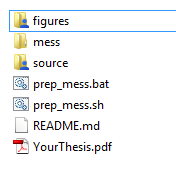
\includegraphics[width=.3\textwidth,keepaspectratio]{dirshot}
    \caption{The same screenshot again, just for demonstration}
    \label{fig:shot2}
\end{figure}

\section{Words of goodbye}
Hope that you find this document useful for you. Please take the good wishes all authors have passed forward and work hard on your research to become a great resource of the world. And again, if you have made things better, please, please make a PULL REQUEST so that future users can enjoy your great contribution. Thanks! Cheers!
 % you can also have one input per chapter


%\appendix % use this if you just have one appendix
%\appendices % use this if you have more than one appendix

%\appendices

%\chapter{First appendix}
%\section*{hidden appendix section}   %  do not show in table of contents

%\chapter{Second appendix}

% put appendices here

% file containing refs if you are not using bibtex
\bibliographystyle{muthesis2017}

\bibliography{references}

\biography % use this to get the biography at the end of the thesis

\end{document}
